\documentclass[11pt,a4paper]{article}

\usepackage[margin=1in]{geometry}
\usepackage{setspace}
\usepackage{booktabs}
\usepackage{array}
\usepackage{longtable}
\usepackage{graphicx}
\usepackage{float}
\usepackage{amsmath}
\usepackage{amssymb}
\usepackage{enumitem}
\usepackage{hyperref}
\usepackage{listings}
\usepackage{xcolor}
\usepackage{tikz}
\usetikzlibrary{arrows.meta,positioning}

\hypersetup{
  colorlinks=true,
  linkcolor=black,
  urlcolor=black,
  citecolor=black
}

\setstretch{1.10}
\setlength{\parskip}{0.2em}
\setlength{\parindent}{0pt}
\setlist[itemize]{topsep=2pt,itemsep=1pt,parsep=0pt,partopsep=0pt}
\setlist[enumerate]{topsep=2pt,itemsep=1pt,parsep=0pt,partopsep=0pt}

\lstdefinestyle{codeblock}{
  basicstyle=\ttfamily\small,
  breaklines=true,
  frame=single,
  backgroundcolor=\color{gray!8}
}

\title{\textbf{DBMS Term Project Report}\\[0.3em]
Implementation of a Page-Backed R-Tree for High-Dimensional Image Indexing}
\author{
Pritam Mondal (23CS30041) \\
Sibashis Som (23CS10091)
}
\date{April 2026}

\begin{document}

\maketitle
\thispagestyle{empty}

\vspace{1em}
\textbf{GitHub Repository:} \url{https://github.com/mpritam17/DBMS-Project}

\textbf{Project Repository Scope:} C++ storage/index engine, Python embedding pipeline, and MERN-based demonstration interface.

\textbf{Source Code Availability:} The complete source code corresponding to this report is provided through the GitHub repository link above.

\tableofcontents
\newpage

\section{Title and Team Members}

\textbf{Project Title:} Implementation of a Page-Backed R-Tree for High-Dimensional Image Indexing

\textbf{Team Members:}
\begin{itemize}[leftmargin=1.5em]
  \item Pritam Mondal -- 23CS30041
  \item Sibashis Som -- 23CS10091
\end{itemize}

\textbf{High-level summary:}

This project presents a disk-oriented similarity-search system for high-dimensional image embeddings. In contrast to purely in-memory indexing approaches, the implementation adheres to DBMS principles through fixed-size page management, explicit storage abstraction, buffer-pool-mediated access, and page-serialized spatial indexing. The system is evaluated against brute-force and KD-tree baselines and is exposed through API and web interfaces for end-to-end demonstration. The pipeline maintains 512D base embeddings and uses PCA projection to 12D for frontend image-similarity workflows and query benchmarks, enabling consistent comparison across R-tree, KD-tree, and brute-force approaches.

\section{Objective}

The objective is to design and validate an end-to-end database-style system for high-dimensional vector search, where data persistence and page-level I/O behavior are first-class concerns.

\subsection{Primary Goals}

\begin{itemize}[leftmargin=1.5em]
  \item Build a page-based storage layer with controlled disk I/O semantics.
  \item Implement a buffer pool manager with replacement strategy suitable for mixed workloads.
  \item Implement a disk-backed R-tree index with insertion, node splits, metadata persistence, and KNN retrieval.
  \item Implement a fixed PCA projection to 12D for frontend similarity and query-benchmark workflows while retaining 512D base embeddings.
  \item Build a reproducible image embedding pipeline that exports vectors into a binary format suitable for bulk loading.
  \item Benchmark query behavior against brute-force and KD-tree baselines.
  \item Provide a demonstration stack (API + UI) for interactive query and image similarity search.
  \item Provide a comparative analysis of trade-offs among R-tree, KD-tree, and brute-force retrieval strategies in a standardized 12D benchmark setting.
\end{itemize}

\subsection{Problem Context}

Traditional one-dimensional indexes (for example B-Tree keyed on scalar values) are not naturally suited for high-dimensional nearest-neighbor search. This project therefore targets spatial/vector indexing with a concrete DBMS architecture:

\begin{itemize}[leftmargin=1.5em]
  \item embeddings and index pages are persisted on disk,
  \item access is mediated through a buffer pool,
  \item performance is evaluated through latency, recall, and I/O counters,
  \item the system is integrated into a demonstration-ready application workflow.
\end{itemize}

\section{Theoretical Background}

\subsection{Principal Component Analysis (PCA)}

Principal Component Analysis is a linear dimensionality-reduction method that projects high-dimensional vectors into a lower-dimensional subspace while preserving maximal variance. For zero-centered data matrix $X \in \mathbb{R}^{n \times d}$, PCA computes eigenvectors of the covariance matrix

\[
\Sigma = \frac{1}{n-1} X^T X.
\]

If the eigenvalues satisfy $\lambda_1 \ge \lambda_2 \ge \cdots \ge \lambda_d$, then selecting the first $m$ eigenvectors forms a projection matrix $W_m$, and each vector is transformed as

\[
z = W_m^T x.
\]

The retained variance ratio is

\[
\text{Retained Variance}(m) = \frac{\sum_{i=1}^{m} \lambda_i}{\sum_{i=1}^{d} \lambda_i}.
\]

In this project, PCA is used to reduce embedding dimensionality before nearest-neighbor search. This reduces storage and computation cost and improves practical query latency, while controlling information loss through variance-retention monitoring. The system keeps base embeddings in 512D and applies PCA projection to 12D for frontend similarity and benchmark execution.

\subsection{R-tree Fundamentals}

An R-tree is a balanced hierarchical spatial index in which each node stores entries represented by Minimum Bounding Rectangles (MBRs). Internal-node entries point to child pages, and leaf-node entries reference object identifiers. Query processing leverages spatial pruning: subtrees whose MBRs cannot improve the current best candidate set are excluded from exploration.

Insertion proceeds by selecting a subtree, descending to a leaf, and applying node splitting upon overflow. In this implementation, quadratic split logic and upward MBR propagation are used to maintain tree consistency. Because the index is page-backed, each structural operation is translated into explicit page reads/writes through the buffer pool.

\subsection{KD-tree Fundamentals}

A KD-tree is a binary space-partitioning structure for point data. Each internal node splits space along one coordinate axis, typically chosen cyclically or by variance, and recursively partitions the dataset into two half-spaces. For low to moderate dimensionality, KD-tree nearest-neighbor search can be efficient due to branch pruning using hyperplane distance bounds.

However, as dimensionality increases, pruning effectiveness degrades (curse of dimensionality), and query behavior may approach brute-force scanning. In this project, KD-tree is used as an in-process baseline to contextualize R-tree and brute-force performance under identical query sets.

\subsection{Comparative Perspective for This Project}

The three methods play distinct roles:

\begin{itemize}[leftmargin=1.5em]
  \item \textbf{R-tree:} page-aware, disk-oriented index aligned with DBMS storage abstractions.
  \item \textbf{KD-tree:} memory-resident geometric baseline with fast behavior at lower dimensions.
  \item \textbf{Brute-force:} exact reference baseline used for recall measurement.
\end{itemize}

This multi-baseline design strengthens interpretation of measured latency and accuracy outcomes.

\section{Methodology}

\subsection{System Architecture}

The implementation follows a modular stack:

\begin{enumerate}[leftmargin=1.7em]
  \item \textbf{Storage Manager} (C++): fixed-size page read/write/allocate/flush primitives.
  \item \textbf{Slotted Page Layer} (C++): variable-length item packing for embedding records.
  \item \textbf{Buffer Pool Manager + Replacer} (C++): in-memory page cache, pin/unpin protocol, and LRU-2 style eviction behavior.
  \item \textbf{R-tree Node and Index Manager} (C++): serialized node format, insertion/splitting, metadata page, KNN and point search.
  \item \textbf{Embedding/Data Pipeline} (Python): image ingestion, ResNet-18 embeddings (512D), PCA projection to 12D for frontend/benchmark workflows, VEC1 export.
  \item \textbf{Query/Integration Layer} (C++ tool + Python/Node APIs): benchmark runner and web-facing endpoints.
  \item \textbf{Frontend Demonstration} (React/Vite): query visualization, image upload search, and benchmark panels.
\end{enumerate}

\subsection{Persistent Data Layout}

\textbf{Page abstraction:}

\begin{itemize}[leftmargin=1.5em]
  \item page size: 16384 bytes,
  \item header size: 64 bytes,
  \item shared page header tracks magic, type, item count, and free-space metadata.
\end{itemize}

\textbf{Embedding store format:}

Each slotted-page item stores:

\[
\texttt{item} = \texttt{uint64\_id} + \texttt{float32[d]}
\]

\textbf{VEC1 bulk-load file format:}

Header layout (24 bytes):

\begin{itemize}[leftmargin=1.5em]
  \item magic (4 bytes): \texttt{VEC1}
  \item version (4 bytes)
  \item vector count (8 bytes)
  \item dimensions (4 bytes)
  \item reserved/flags (4 bytes)
\end{itemize}

Record layout:

\[
\texttt{record} = \texttt{uint64\_id} + \texttt{float32[d]}
\]

This design enables simple, deterministic transfer from Python feature extraction to C++ storage/index loading.

\subsection{Buffer Pool and Replacement Policy}

The buffer pool manager maintains page frames, page-to-frame mapping, free list, and replacement structure. Important implementation choices:

\begin{itemize}[leftmargin=1.5em]
  \item zero-copy page I/O methods for direct read/write into frame buffers,
  \item metadata lock scope reduction so disk I/O happens outside the global BPM latch,
  \item frame pin/unpin protocol integrated with replacer state transitions,
  \item fetch statistics (requests, hits, misses, hit-rate) exposed for benchmark reporting.
\end{itemize}

Replacement strategy is LRU-2 inspired:

\begin{itemize}[leftmargin=1.5em]
  \item first touch enters FIFO queue,
  \item repeated touches move to hot LRU queue,
  \item eviction prefers one-touch pages first, reducing scan pollution effect on hot pages.
\end{itemize}

\subsection{R-tree Index Implementation}

\textbf{Node serialization:}

Each R-tree node is serialized inside one page with:

\begin{itemize}[leftmargin=1.5em]
  \item shared 64-byte page header,
  \item 32-byte node header (dimensions, entry count, parent link, leaf link),
  \item fixed-size entries: lower bounds + upper bounds + value/child pointer.
\end{itemize}

For dimension $d$, entry size is:

\[
\texttt{entry\_bytes} = 2d \cdot \texttt{sizeof(float)} + \texttt{sizeof(uint64)}
\]

At $d=128$:

\[
\texttt{entry\_bytes} = 2 \cdot 128 \cdot 4 + 8 = 1032
\]

With 16KB pages, this gives a practical branching factor (15 entries/page).

\textbf{Insertion and split strategy:}

\begin{itemize}[leftmargin=1.5em]
  \item recursive descent to leaf,
  \item quadratic split when overflow occurs,
  \item upward MBR propagation,
  \item root growth when split reaches root.
\end{itemize}

\textbf{High-dimensional numerical stability fix:}

A key issue in 128D is hyper-volume underflow if using direct edge-product volume calculations. To avoid subtree-choice collapse, subtree selection uses log-space enlargement ratio:

\[
\log\left(\frac{V_{\text{expanded}}}{V_{\text{original}}}\right)
= \sum_i \log\left(\frac{\Delta_i^{\text{expanded}}}{\Delta_i^{\text{original}}}\right)
\]

This preserves relative ordering without underflow to zero.

\subsection{KNN and Point Search Strategy}

KNN query uses branch-and-bound traversal:

\begin{itemize}[leftmargin=1.5em]
  \item min-heap keyed by lower-bound distance from query to node MBR,
  \item max-heap of current top-$k$ candidate results,
  \item global pruning when best frontier bound cannot improve current $k$th distance.
\end{itemize}

Distance lower bound to MBR is:

\[
\text{MinDist}^2(q, B) = \sum_i
\begin{cases}
(l_i - q_i)^2, & q_i < l_i \\
(q_i - u_i)^2, & q_i > u_i \\
0, & l_i \le q_i \le u_i
\end{cases}
\]

Point-search endpoint is also implemented, returning exact coordinate matches and diagnostics (nodes visited, entries examined).

\subsection{Query Benchmark Methodology}

The query benchmark tool performs:

\begin{enumerate}[leftmargin=1.7em]
  \item read vectors from slotted-page embedding store,
  \item build/reuse companion index database (\texttt{<db>.rtree\_tmp.db}),
  \item run R-tree KNN,
  \item run in-process KD-tree baseline,
  \item run brute-force baseline,
  \item compute recall@k and fetch/I/O counters,
  \item optionally export per-query CSV rows.
\end{enumerate}

The benchmark workflow uses 12D PCA-projected vectors derived from 512D embeddings, enabling direct latency and recall comparison among R-tree, KD-tree, and brute-force baselines in a fixed-dimensional setting.

Recall metric:

\[
\text{Recall@k} = \frac{|\text{ApproxTopK} \cap \text{ExactTopK}|}{|\text{ExactTopK}|}
\]

\subsection{Image Dataset for Similarity Search (CIFAR-10)}

The image-similarity feature is developed and evaluated primarily on CIFAR-10, a widely used benchmark dataset containing 60000 color images of size $32 \times 32$ distributed across 10 semantic classes: airplane, automobile, bird, cat, deer, dog, frog, horse, ship, and truck.

For this project, both training and test splits are used to construct a unified retrieval corpus (up to 60000 images), enabling large-scale similarity experiments while preserving class diversity. During preprocessing, each image is converted to RGB, resized for the embedding backbone input, and transformed into 512D feature vectors, followed by PCA projection to 12D for frontend similarity and benchmark workloads.

CIFAR-10 is suitable for this system for three reasons:

\begin{itemize}[leftmargin=1.5em]
  \item it provides a standard, reproducible benchmark for comparative evaluation,
  \item it has sufficient scale for observing index and cache behavior,
  \item class diversity supports qualitative and quantitative validation of nearest-neighbor retrieval quality.
\end{itemize}

Although retrieval itself is vector-distance based and label-agnostic at query time, class labels are useful for interpreting whether returned neighbors are semantically consistent.

\subsection{Image Search and MERN Integration}

The demonstration stack combines:

\begin{itemize}[leftmargin=1.5em]
  \item Flask image extraction service (ResNet-18 + projection + optional PCA),
  \item Express backend orchestrating benchmark binary/API requests,
  \item React frontend with image upload search and query benchmark tabs.
\end{itemize}

Recent integration-level workflow includes:

\begin{itemize}[leftmargin=1.5em]
  \item image upload based query path,
  \item optional near-duplicate shortcut by hash,
  \item incremental insert endpoint (image to embedding to append to store + index update),
  \item API-level diagnostics for point search and KNN timing.
\end{itemize}

\subsection{Validation and Test Coverage}

C++ tests validate:

\begin{itemize}[leftmargin=1.5em]
  \item storage smoke behavior,
  \item slotted-page packing and reload integrity,
  \item buffer pool eviction/flush semantics,
  \item R-tree node serialization and 128D capacity,
  \item insertion, split, and tree consistency,
  \item KNN correctness versus brute-force checks,
  \item metadata persistence and reopen behavior.
\end{itemize}

This test-driven workflow reduces behavioral regression risk while evolving the project from week 1 to week 5 scope.

\section{Tech Stack}

\subsection{Languages and Core Development Environment}

\begin{itemize}[leftmargin=1.5em]
  \item \textbf{C++17:} storage engine, buffer manager, index structures, and benchmark executables.
  \item \textbf{Python 3:} embedding generation, PCA utilities, vector-format validation, and baseline comparison scripts.
  \item \textbf{JavaScript (Node.js/React):} backend orchestration and frontend demonstration interfaces.
\end{itemize}

\subsection{Libraries, Frameworks, and Tools}

\begin{itemize}[leftmargin=1.5em]
  \item \textbf{Build System:} CMake.
  \item \textbf{ML and Data:} PyTorch, TorchVision, NumPy, scikit-learn, Pillow.
  \item \textbf{API Services:} Flask, Flask-CORS, Express.js, Multer.
  \item \textbf{Persistence/Logging:} custom page store and optional MongoDB via Mongoose.
  \item \textbf{Frontend:} React and Vite.
  \item \textbf{Baseline DB:} SQLite.
\end{itemize}

\subsection{Layer-wise Stack Mapping}

\begin{table}[H]
\centering
\caption{Technology mapping by system layer}
\begin{tabular}{p{0.28\textwidth}p{0.62\textwidth}}
\toprule
System Layer & Technology \\
\midrule
Storage and index engine & C++17, custom Storage Manager, Slotted Page, Buffer Pool, R-tree modules \\
Build and compilation & CMake \\
Embedding and dimensionality reduction & PyTorch, TorchVision, NumPy, scikit-learn PCA, Pillow \\
Benchmark and evaluation & C++ query benchmark tool, Python analysis scripts, SQLite baseline \\
Service/API integration & Flask image API, Express.js orchestrator, optional MongoDB/Mongoose \\
User interface & React + Vite frontend \\
\bottomrule
\end{tabular}
\end{table}

\section{Changes from the Original Proposal}

The original proposal established the intended DBMS architecture and weekly milestones. During implementation, several modifications were introduced to improve correctness, scalability, and reproducibility. These changes are summarized in Table~\ref{tab:proposal-changes}, together with the motivation and concrete benefits.

\begin{table}[H]
\centering
\caption{Changes from proposal with rationale and improvement}
\label{tab:proposal-changes}
\begin{tabular}{p{0.23\textwidth}p{0.23\textwidth}p{0.23\textwidth}p{0.23\textwidth}}
\toprule
Original Proposal Assumption & Implemented Change & Reason for Change & Improvement / Error Fixed \\
\midrule
4KB pages as default physical granularity & Increased effective page capacity for index workload (16KB pages in current implementation) & 4KB pages yielded low branching factor in high dimensions and weak KNN pruning & Higher fan-out, reduced tree height, and improved branch-and-bound effectiveness \\
\midrule
Standard volume-based subtree enlargement for insertion & Adopted log-space enlargement ratio for subtree selection & Direct high-dimensional volume products underflowed numerically, degrading child selection quality & Numerically stable decisions, improved tree balance, reduced overlap-related inefficiency \\
\midrule
Generic cache replacement behavior & Implemented LRU-2 style replacement and reduced global latch hold during disk I/O & Mixed hot-set + scan workloads caused cache pollution and lock-scope overhead & Better hot-page retention and improved robustness of buffer-pool behavior under mixed access patterns \\
\midrule
Single-file conceptual index/data coupling & Introduced companion index database file (\texttt{<db>.rtree\_tmp.db}) & Isolating index pages from embedding pages simplified rebuild and reduced corruption risk during iteration & Safer recovery path and faster experimental iteration without rewriting source vectors \\
\midrule
In-memory root/index state tracked by process & Added explicit metadata page and reopen path for persisted indexes & Reopen correctness required durable metadata rather than process-local state & Reliable index reloading across process restarts and improved persistence semantics \\
\midrule
Core comparison against brute-force and SQLite only & Added KD-tree baseline and point-search diagnostics in benchmark workflow & Additional baseline and diagnostics were needed for clearer interpretation of recall/latency trade-offs & More informative evaluation and stronger validation of query-layer behavior \\
\midrule
Initial dimensionality control was considered for user-driven runtime changes & Standardized to 512D base embeddings with fixed PCA projection to 12D for frontend and benchmark paths & Runtime dimension switching increases interface complexity and weakens experiment reproducibility across runs & Provides stable, repeatable, and fair comparison of R-tree, KD-tree, and brute-force while preserving high-dimensional source representations \\
\midrule
Initial dataset/ID pipeline assumptions & Added deterministic seeding and robust ID mapping for large-scale (up to 60000 image) pipelines & Non-deterministic transformations and ID-order issues reduced reproducibility and traceability & Stable experiments, consistent ID-to-image correspondence, and cleaner benchmarking \\
\bottomrule
\end{tabular}
\end{table}

These refinements preserve the proposal's original objective while resolving implementation-time inefficiencies and correctness risks discovered through testing.

\section{Results and Screenshots}

\subsection{Implementation Outcome}

The repository demonstrates an end-to-end, page-aware vector search system that includes:

\begin{itemize}[leftmargin=1.5em]
  \item persistent storage for vector records,
  \item buffer-pooled page access,
  \item page-backed R-tree with metadata persistence,
  \item query benchmarking against multiple baselines,
  \item application-level image query interface and API integration.
\end{itemize}

\subsection{Documented Performance Results (Repository-Recorded)}

\textbf{A. Buffer-pool benchmark summary (Week 2 notes):}

\begin{table}[H]
\centering
\caption{Saved benchmark artifacts for BPM optimization set}
\begin{tabular}{lrrr}
\toprule
Run & Total Time (ms) & Disk Reads & Relative Read Change \\
\midrule
Baseline & 202.829 & 10294 & -- \\
Optimized & 243.666 & 9794 & -4.86\% \\
Optimized Final & 290.541 & 9791 & -4.89\% \\
\bottomrule
\end{tabular}
\end{table}

Interpretation: disk-read penalties consistently dropped by about 5\%, but the available saved timings do not yet show a stable wall-clock speedup for that specific mixed workload.

\textbf{B. R-tree high-dimensional structural gains (Week 3 notes):}

\begin{table}[H]
\centering
\caption{Impact of page-size update for 128D entries}
\begin{tabular}{lcc}
\toprule
Metric & 4KB Page & 16KB Page \\
\midrule
Entries per page at 128D & 3 & 15 \\
Effective branching factor & 3 & 15 \\
Approx. tree height (50 vectors) & 4 & 2 \\
Pruning opportunity in KNN & low & high \\
\bottomrule
\end{tabular}
\end{table}

Interpretation: larger page capacity significantly improves fan-out and pruning behavior in KNN traversal.

\textbf{C. Dataset and embedding pipeline progression (Week 5 notes):}

\begin{itemize}[leftmargin=1.5em]
  \item scaling from small samples to 60000 CIFAR-10 images,
  \item maintenance of 512D base embeddings with fixed PCA projection to 12D for frontend similarity and benchmark workflows,
  \item standardized latency/recall comparison across R-tree, KD-tree, and brute-force in a fixed-dimensional setup,
  \item compact 12D operational representation for interactive similarity querying,
  \item deterministic projector initialization for repeatable embedding behavior.
\end{itemize}

\subsection{Milestone Completion Mapping}

\begin{table}[H]
\centering
\caption{Planned milestones vs implemented outcomes}
\begin{tabular}{p{0.24\textwidth}p{0.67\textwidth}}
\toprule
Planned Milestone & Implemented Outcome \\
\midrule
Week 1: Storage + data pipeline & Storage manager, VEC1 export/validation, slotted-page packing, bulk load path completed. \\
Week 2: Buffer pool + serialization & BPM with latch/refetch logic, LRU-2 style replacer, zero-copy I/O path and benchmark harness completed. \\
Week 3: Index + KNN & R-tree node serialization, insertion/split, metadata page, KNN and point-search implementations with tests completed. \\
Week 4: Integration + benchmarking & Unified query benchmark tool, CSV export, KD/brute baselines, recall and I/O metrics reporting completed. \\
Week 5: End-to-end demo & MERN + Flask image-query integration, incremental insert path, larger dataset workflow, and fixed 12D PCA projection over 512D embeddings for frontend and benchmark workflows completed. \\
\bottomrule
\end{tabular}
\end{table}

\subsection{Screenshots for Final Demonstration}

The following figure placeholders are included to satisfy the report screenshot requirement. Replace each placeholder with actual images captured from your local run.

\begin{figure}[H]
\centering
\resizebox{0.98\textwidth}{!}{%
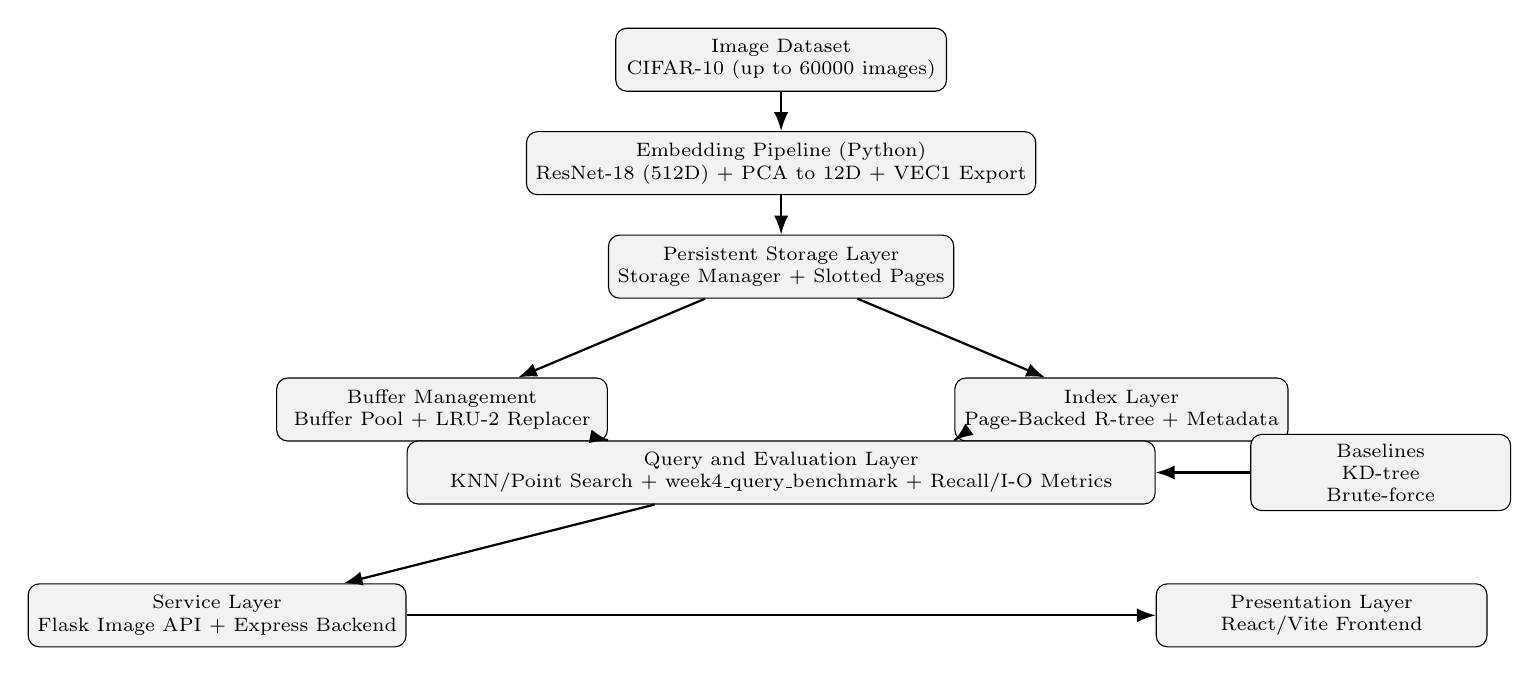
\begin{tikzpicture}[
  node distance=5mm and 6mm,
  box/.style={
    draw,
    rounded corners,
    align=center,
    minimum height=8mm,
    minimum width=42mm,
    font=\scriptsize,
    fill=gray!10
  },
  arrow/.style={-{Latex[length=2.4mm]}, thick}
]
  \node[box] (data) {Image Dataset\\CIFAR-10 (up to 60000 images)};
  \node[box, below=of data] (embed) {Embedding Pipeline (Python)\\ResNet-18 (512D) + PCA to 12D + VEC1 Export};
  \node[box, below=of embed] (store) {Persistent Storage Layer\\Storage Manager + Slotted Pages};

  \node[box, below left=10mm and 0mm of store] (bpm) {Buffer Management\\Buffer Pool + LRU-2 Replacer};
  \node[box, below right=10mm and 0mm of store] (rtree) {Index Layer\\Page-Backed R-tree + Metadata};

  \node[box, below=18mm of store, minimum width=95mm] (query) {Query and Evaluation Layer\\KNN/Point Search + week4\_query\_benchmark + Recall/I-O Metrics};
  \node[box, below left=10mm and 0mm of query] (api) {Service Layer\\Flask Image API + Express Backend};
  \node[box, below right=10mm and 0mm of query] (ui) {Presentation Layer\\React/Vite Frontend};
  \node[box, right=12mm of query, minimum width=33mm] (base) {Baselines\\KD-tree\\Brute-force};

  \draw[arrow] (data) -- (embed);
  \draw[arrow] (embed) -- (store);
  \draw[arrow] (store) -- (bpm);
  \draw[arrow] (store) -- (rtree);
  \draw[arrow] (bpm) -- (query);
  \draw[arrow] (rtree) -- (query);
  \draw[arrow] (base) -- (query);
  \draw[arrow] (query) -- (api);
  \draw[arrow] (api) -- (ui);
\end{tikzpicture}%
}
\caption{System architecture used in the implementation}
\label{fig:architecture}
\end{figure}

\begin{figure}[H]
\centering
\fbox{\parbox[c][2.2in][c]{0.88\textwidth}{\centering
Screenshot Placeholder 2\\
Frontend image search tab showing uploaded image, neighbors, and timings
}}
\caption{Image search UI demonstration}
\label{fig:image-search-ui}
\end{figure}

\begin{figure}[H]
\centering
\includegraphics[width=0.88\textwidth]{benchmarking.png}
\caption{Query benchmark UI and diagnostics}
\label{fig:query-ui}
\end{figure}

\subsection{Guide to Run the Project}

This section provides a practical execution sequence for reproducing the implemented pipeline and demonstration workflow.

\textbf{1. Install Python dependencies}

\begin{lstlisting}[style=codeblock]
python -m venv .venv
.venv\Scripts\activate
python -m pip install -r requirements.txt
\end{lstlisting}

\textbf{2. Configure and build C++ components}

\begin{lstlisting}[style=codeblock]
cmake -S . -B build
cmake --build build
\end{lstlisting}

\textbf{3. (Optional) Generate dataset vectors and load embedding store}

\begin{lstlisting}[style=codeblock]
python scripts/populate_database.py --source cifar10 --count 60000 --pca-dims 12
# fixed projection for frontend and benchmark workflow
# use --pca-dims 12
./build/bulk_load data/sample_vecs.bin sample.db
\end{lstlisting}

\textbf{4. Run the query benchmark}

\begin{lstlisting}[style=codeblock]
./build/week4_query_benchmark sample.db all:200 10 benchmark_week4.csv
# run comparison in standardized 12D working space (from 512D embeddings)
\end{lstlisting}

\textbf{5. Start image extraction API (Flask)}

\begin{lstlisting}[style=codeblock]
python scripts/image_search_api.py --vec-file data/sample_vecs.bin --image-dir data/sample_images
\end{lstlisting}

\textbf{6. Start MERN backend}

\begin{lstlisting}[style=codeblock]
cd mern/backend
npm install
npm run dev
\end{lstlisting}

\textbf{7. Start MERN frontend}

\begin{lstlisting}[style=codeblock]
cd mern/frontend
npm install
npm run dev
\end{lstlisting}

\textbf{8. Verify from browser}

Open the frontend URL reported by Vite (typically \texttt{http://localhost:5173}) and execute:

\begin{itemize}[leftmargin=1.5em]
  \item image-based similarity query,
  \item vector-id benchmark query,
  \item incremental insert and post-insert re-query validation.
\end{itemize}

\subsection{Limitations and Next Steps}

\begin{itemize}[leftmargin=1.5em]
  \item Stronger transactional guarantees and crash recovery are future improvements.
  \item Benchmark isolation can be improved to separate lock-contention effects from cache-policy effects.
  \item Additional large-scale and repeated-run experiments should be automated into CI artifacts.
  \item A formal visual dashboard for benchmark trend analysis can improve reporting quality.
\end{itemize}

\section{References}

\begin{thebibliography}{99}

\bibitem{proposal}
DBMS Project Proposal (group submission), March 2026.

\bibitem{repo-readme}
Project README and implementation documents:
\texttt{README.md},
\texttt{docs/WEEK1\_IMPLEMENTATION\_DETAILS.md},
\texttt{docs/WEEK2\_PERFORMANCE.md},
\texttt{docs/WEEK3\_INDEX\_FOUNDATION.md},
\texttt{docs/WEEK4\_QUERY\_LAYER.md},
\texttt{docs/WEEK5\_IMAGE\_SEARCH\_AND\_MERN.md}.

\bibitem{guttman1984}
Antonin Guttman.
\textit{R-Trees: A Dynamic Index Structure for Spatial Searching}.
Proceedings of ACM SIGMOD, 1984.

\bibitem{resnet}
Kaiming He, Xiangyu Zhang, Shaoqing Ren, Jian Sun.
\textit{Deep Residual Learning for Image Recognition}.
CVPR, 2016.

\bibitem{cifar10}
Alex Krizhevsky.
\textit{Learning Multiple Layers of Features from Tiny Images}.
Technical Report, 2009.

\bibitem{sqlite}
SQLite Documentation.
\url{https://www.sqlite.org/docs.html}

\bibitem{pytorch}
PyTorch Documentation.
\url{https://pytorch.org/docs/stable/index.html}

\bibitem{mongodb}
MongoDB Documentation.
\url{https://www.mongodb.com/docs/}

\bibitem{react}
React Documentation.
\url{https://react.dev/}

\bibitem{jolliffe2002}
Ian T. Jolliffe.
\textit{Principal Component Analysis}.
Springer, 2nd edition, 2002.

\bibitem{bentley1975}
Jon Louis Bentley.
\textit{Multidimensional Binary Search Trees Used for Associative Searching}.
Communications of the ACM, 18(9):509--517, 1975.

\end{thebibliography}

\end{document}
